\documentclass[mathserif]{beamer}

\usepackage{graphicx}
\usepackage{hyperref}
\usepackage{amsmath}
\usepackage{changepage}
\usepackage{bbm}

\usetheme{Berlin}
\usecolortheme{beetle}
\beamertemplatenavigationsymbolsempty 



%%%%%% Column Layout %%%%%%%%%%%%
%	\begin{columns}
%		\begin{column}{.5\textwidth}
%			
%		\end{column}
%		\begin{column}{.5\textwidth}
%			
%		\end{column}
%	\end{columns}


\title[How Much is too Much? -- Beliefs about Perceived Inequality in a Coordination Game]{How Much is too Much?\\
	Beliefs about Perceived Inequality in a Coordination Game}
\author{Tim Schulz}
\institute[SFU]
{
	Simon Fraser University\\
	Department of Economics
}
\date{August 2, 2016}


\begin{document}
	\frame{\titlepage}
	\section{Motivation}
	\begin{frame}{Motivation}
		History:
		\begin{itemize}
			\item many successful revolutions when inequality ``got out of hand"
			\item many failed revolutions (e.g. Arab Spring)
		\end{itemize}
		\pause
		Hypotheses about the future:
		\begin{itemize}
			\item Piketty: ``Capital in the Twenty-First Century"
		\end{itemize}
	\end{frame}
	
	\section{Goals}
	\begin{frame}{Goals}
		Describe how...
		\begin{itemize}[<+->]
			\item poor perceive inequality
			\begin{itemize}
				\item When do I believe that other poor people decide to revolt against inequality?
				\item For what levels of inequality do I believe that rich people think there may be a problem and start ``defending" against a possible revolution?
			\end{itemize}
			\item rich perceive inequality
			\begin{itemize}
				\item What levels of inequality do I believe poor people will accept?
				\item When do I start worrying about possible adverse consequences of inequality and try to insure myself against revolutions?
			\end{itemize}
			\item success of coordination depends on observed inequality
		\end{itemize}
	\end{frame}
	
	\section{Model}
	\subsection{Payoffs}
	\begin{frame}{Payoffs}
		What determines inequality?\\
		-- Inequality in possible payoffs
		
		\pause
		\textbf{Payoffs for poor players:}
		\begin{adjustwidth*}{-1cm}{-1cm}
		\begin{table}[!htbp]
			\caption{General Payoffs of Poor}
			\label{table:gpayoff}
			\begin{center}
				\begin{tabular}{|l|c|c|c|l|c|c|}
					\multicolumn{3}{c}{Under \texttt{no insurance} $(n)$} &
					\multicolumn{1}{c}{} &
					\multicolumn{3}{c}{Under \texttt{insurance} $(i)$}\\
					\cline{1-3}\cline{5-7}
					& revolt & do nothing & & & revolt & do nothing\\
					\cline{1-3}\cline{5-7}
					revolt & $h_n, h_n$ & $l_n, m_n$ && revolt & $h_i, h_i$ & $l_i, 
					m_i$\\
					\cline{1-3}\cline{5-7}
					do nothing & $m_n, l_n$ & $m_n, m_n$ && do nothing & $m_i, l_i$ & 
					$m_i, m_i$\\
					\cline{1-3}\cline{5-7}
				\end{tabular}
			\end{center}
					\footnotesize
					Payoffs of poor players depending on the other poor player's decision 
					and depending on whether the rich person opted for insurance. 
		\end{table}
		\end{adjustwidth*}
	\end{frame}
	
	\begin{frame}
		Some simplifications:
		
		\begin{itemize}
			\item $h_n=h_i=h$
			\item $m_n=m_i=m$
		\end{itemize}
		
		\pause
		\begin{table}[!htbp]
			\caption{Simplified Payoffs of Poor}
			\label{spayoff}
			\centering
			\begin{tabular}{|l|c|c|}
				\hline
				& revolt & do nothing\\
				\hline
				revolt & $h, h$ & $l_j, m$\\
				\hline
				do nothing & $m, l_j$ & $m, m$\\
				\hline
			\end{tabular}\\
			\footnotesize Where $j\in\{i, n\}$ and $l_n>l_i$.
		\end{table}
	\end{frame}
	
	\begin{frame}{Payoffs}
		\textbf{Payoffs for rich players}
		
		\begin{adjustwidth*}{-1cm}{-1cm}
		\begin{table}[!htbp]
			\caption{Payoffs of Rich}
			\label{rpayoffs}
			\centering
			\begin{tabular}{|c||c|c|c|c||c|c|}
				\multicolumn{3}{c}{General Form} &
				\multicolumn{1}{c}{} &
				\multicolumn{3}{c}{Simplified Form}\\
				\cline{1-3}\cline{5-7}
				number of & & no & & number of & & no\\
				revolts & insurance & insurance && revolts & 
				insurance & insurance\\
				\cline{1-3}\cline{5-7}
				0 & $y_{0i}$ & $y_{0n}$ && 0 & $y_{fi}$ & $y_{0n}$\\
				\cline{1-3}\cline{5-7}
				1 & $y_{1i}$ & $y_{1n}$ && 1 & $y_{fi}$ & $y_{1n}$\\
				\cline{1-3}\cline{5-7}
				2 & $y_{2i}$ & $y_{2n}$ && 2 & $y_2$ & $y_2$\\
				\cline{1-3}\cline{5-7}
			\end{tabular}
		\end{table}
	\end{adjustwidth*}
	
	where 
	 $$y_{0n} > y_{0i}=y_{1i}=y_{fi} > y_{1n} > y_{2i}=y_{2n}=y_2$$
	\end{frame}
	
	\subsection{Decisions}
	\begin{frame}{Decision Making Process -- Rich}
		$\gamma$ -- the believed probability of a poor person revolting
		
		\pause
		A rich person believes that
		\begin{itemize}[<+->]
			\item nobody revolts with probability $(1-\gamma)^2$
			\item 1 poor player revolts with probability $2\gamma(1-\gamma)$
			\item both poor players revolt with probability $\gamma^2$
		\end{itemize}
		\pause
		Then, a rich person purchases insurance if
		\begin{align*}
			\left[(1-\gamma)^2 + 2\gamma(1-\gamma)\right]y_{fi} + \gamma^2y_2 &\geq 
			(1-\gamma)^2y_{0n} + 2\gamma(1-\gamma)y_{1n} + \gamma^2y_2\\
			\gamma &\geq \frac{y_{0n} - y_{fi}}{y_{fi} + y_{0n} -2y_{1n}} \equiv 
			\gamma_1.
		\end{align*}
	\end{frame}
	
	\begin{frame}{Decision Making Process -- Poor}
		$\delta$ -- the believed probability of a rich person having insurance
		
		\pause
		A rational poor person will choose to revolt if
		$$\gamma h + (1-\gamma)\left[ (1-\delta)l_n + \delta l_i \right] \geq m $$
		
		\pause
		Assume I believe there is insurance ($\gamma>\gamma_1$): Revolt if 
		\begin{align*}
			\gamma h + (1-\gamma)l_i &\geq m\\
			\gamma &\geq \frac{m-l_i}{h-l_i} \equiv \gamma_2
		\end{align*}
		
		\pause
		Assume I believe there is no insurance ($\gamma<\gamma_1$):	Revolt if
		\begin{align*}
			\gamma h + (1-\gamma)l_n &\geq m\\
			\gamma &\geq \frac{m-l_n}{h-l_n} \equiv \gamma_3
		\end{align*}
	\end{frame}
	
	\subsection{Outcomes}
	\begin{frame}{Possible outcomes of the game}
		4 possible outcomes:
		\begin{itemize}[<+->]
			\item no insurance, no revolution
			\item no insurance, revolution
			\item insurance, no revolution
			\item insurance, revolution
		\end{itemize}
		\pause
		Only way to rationally allow for all 4 outcomes: Arrange payoffs such that
		$$0 \leq \gamma_3 < \gamma_1 < \gamma_2 \leq 1$$
	\end{frame}
	
	\section{Experiment}
	\begin{frame}{The Experiment}
		\begin{itemize}[<+->]
			\item $2\times2\times3$ design
			\begin{itemize}
				\item randomly assigned to role of rich or poor player
				\item low or high (internal) risk
				\item low, medium or high inequality
			\end{itemize}
			\item groups of 3 (2 poor, 1 rich)
			\item 30 rounds
			\item random order of treatments
		\end{itemize}
	\end{frame}
	
	\begin{frame}
		\begin{table}[!htbp]
			\caption{Payoff Treatments}
			\label{allpayoffs}
			\centering
			\begin{tabular}{|c|c||c|c|c|c||c|c|c|}
				\multicolumn{2}{c}{Treatment} &\multicolumn{7}{c}{Payoffs}\\
				\hline
				Risk & Inequality & $l_i$ & $l_n$ & $m$ & $h$ & $y_{1n}$ & $y_{fi}$ 
				& $y_{on}$\\
				\hline
				low & low & 130 & 280 & 440 & 750 & 490 & 1100 & 1820\\
				low & medium & 130 & 280 & 440 & 750 & 980 & 2200 & 3640\\
				low & high & 130 & 280 & 440 & 750 & 1960 & 4400 & 7280\\
				high & low & 75 & 130 & 320 & 750 & 500 & 2250 & 4000\\
				high & medium & 75 & 130 & 320 & 750 & 1000 & 4500 & 8000\\
				high & high & 75 & 130 & 320 & 750 & 2000 & 9000 & 16000\\			
				\hline
			\end{tabular}
		\end{table}
	\end{frame}
	
	\begin{frame}{What a round looks like}
		\begin{enumerate}[<+->]
			\item participants are randomly selected into groups of three and randomly assigned to the role of rich or poor person
			\item all players are informed about everybody's endowment
			\item all players are informed about everybody's payoff tables
			\item poor players choose whether to revolt
			\item rich players indicate if they believe a successful revolution to occur and decide whether to buy insurance
			\item all players are informed about the number of revolutionaries, the existence of insurance, and their respective payoffs
			\item payment for 3 randomly selected periods (\$1 per 1000 points)
		\end{enumerate}
	\end{frame}
	
	\section{Simulation}
	\begin{frame}{Simulation Study}
		Some deviations from the experiment:
		\begin{itemize}[<+->]
			\item no switching between the roles of poor and rich players
			\item (near) continuum of treatments (1,707 different payoff allocations)
			\item 500 rounds
			\item observable: $d=1-\frac{m}{y_{0n}}$ as a measure of inequality
		\end{itemize}
	\end{frame}
	
	\begin{frame}
		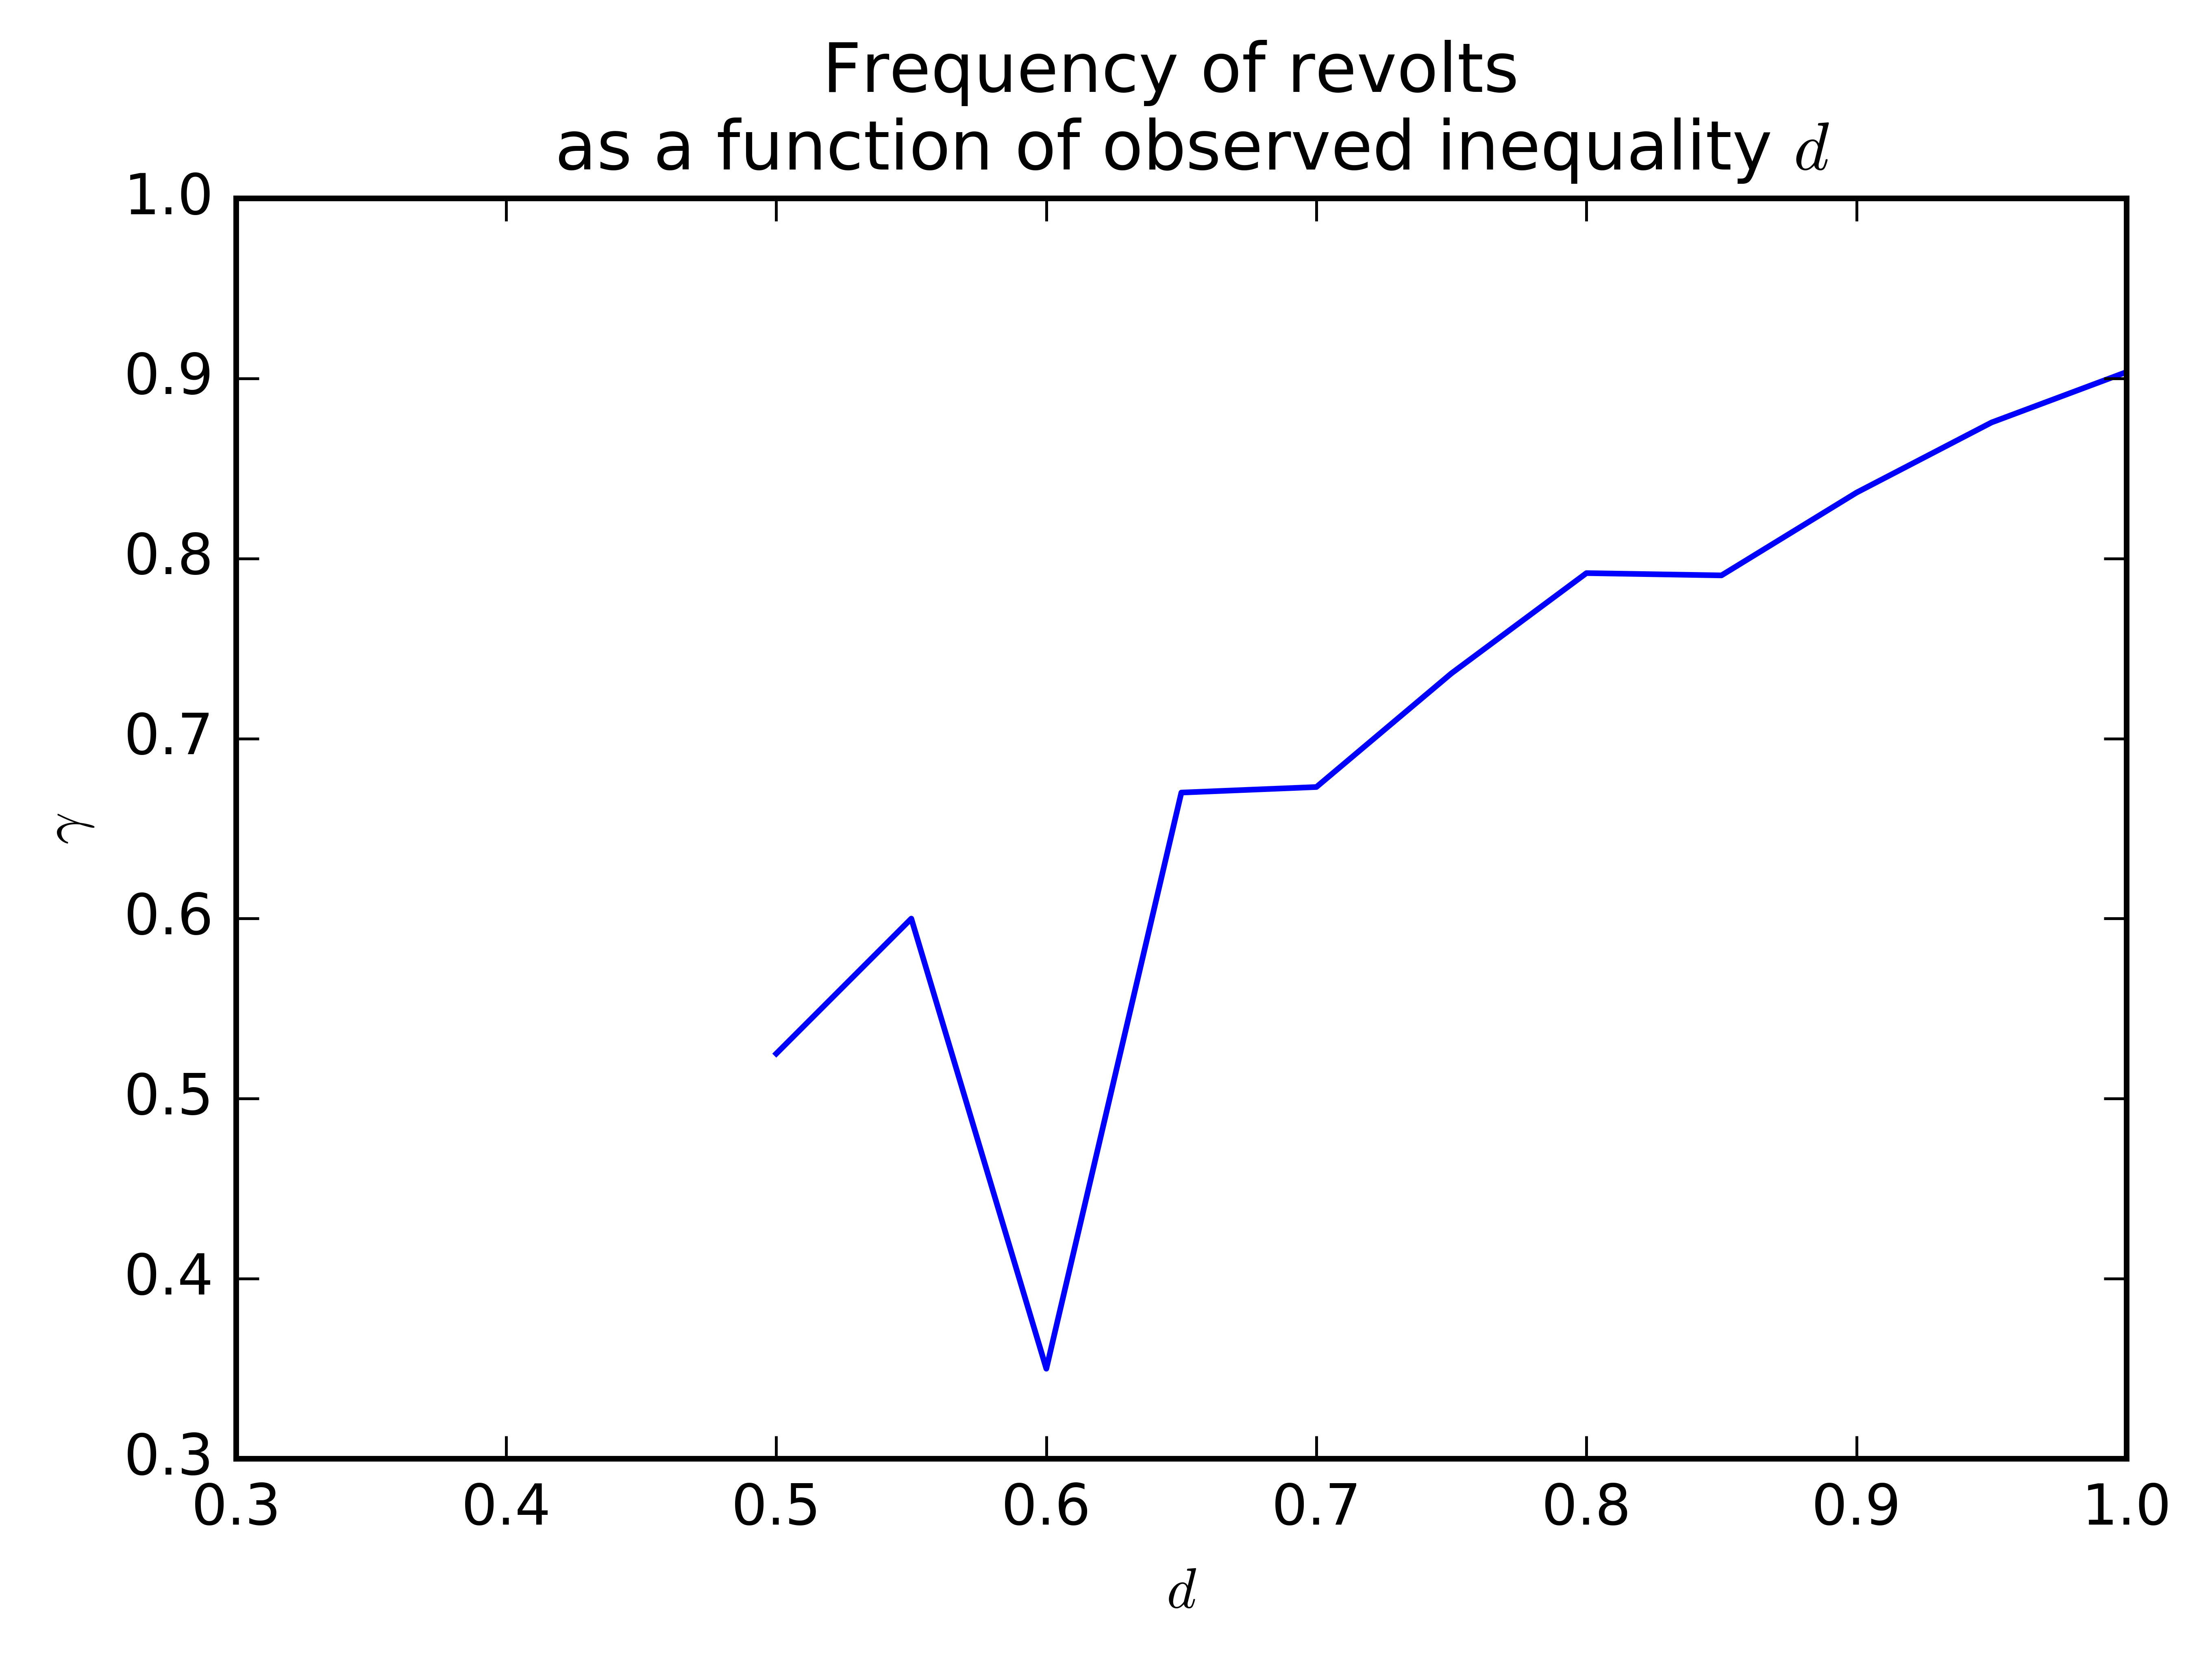
\includegraphics[height=\textheight]{../graph.png}
	\end{frame}
	
	\section{Analysis}
	\begin{frame}{Analysis}
		Calculate $\gamma$ from rich players' frequency of believing in a successful revolution ($\gamma^2$)
		
		\pause
		\begin{align*}
			\gamma_{it} = b_0 &+ b_1\mathbbm{1}\{inequality_t=medium\}\\
			&+ b_2\mathbbm{1}\{inequality_t=high\}\\
			&+ b_3\mathbbm{1}\{role_t=rich\}\\
			&+ b_4\mathbbm{1}\{risk_t=high\} + \kappa_i + \epsilon_{it}
		\end{align*}
	\end{frame}
	
	\section{Hypotheses}
	\begin{frame}{Some Initial Hypotheses}
		\begin{itemize}[<+->]
			\item $0<b_1<b_2$: higher inequality $\implies$ higher probability of revolution
			\item $b_3<0$: rich perceive inequality as less significant than poor
			\item $b_4$ not immediately clear, mostly as control variable
		\end{itemize}
	\end{frame}

\end{document}